\subsection{Product perspective}
TrackMe is a system which has to be designed as a completely new platform. It can be divided into 
two parts: a software application designed for the stakeholders (e.g. users, third parties, ...) and a 
core system interacting with the application via Internet. 
\par
The former one is intended to be a mobile application which requires, necessarily, other devices to work 
as expected by the functionality defined in the Product functions section. For instance, a possible gear 
to interact with the mobile application is a smartwatch, which helps, mainly, the application to 
gather information about the user's health data. Another essential requirement for the application to 
work is to have a stable connection to the Internet; without this obligation, the core system cannot 
collect information about the user. All these requirements are not essentials for third party users.
\par
The latter system has to provide a central connection for every user. The most important object, that has 
to be regarded as a core, is the data. Overall, the TrackMe system is designed to share data and 
information about users. Therefore, a Data Storage System (DSS) is necessary and enables the 
core application to be able to save data and share it when asked. For instance, the DSS can be a 
database that can be accessed through standard interfaces, such as JDBC. Another essential 
requirement for the system is to safeguard the data collected; during the connection between the 
mobile application and the core system, TrackMe has to guarantee that nobody is tracing their data. 
Therefore, it is necessary to use some sort of strong network security, such as SSL/TLS protocols. 
Furthermore functionality of AutomatedSOS and Track4Run are satisfied by using APIs of other companies 
(e.g. Google API for maps and voice recognition).
\\\par
Regarding the environment of the TrackMe system, the following diagram (Figure: \ref{fig:classdiagram}) 
is provided to describe better the domain model adopted:\\

\begin{figure}[H]
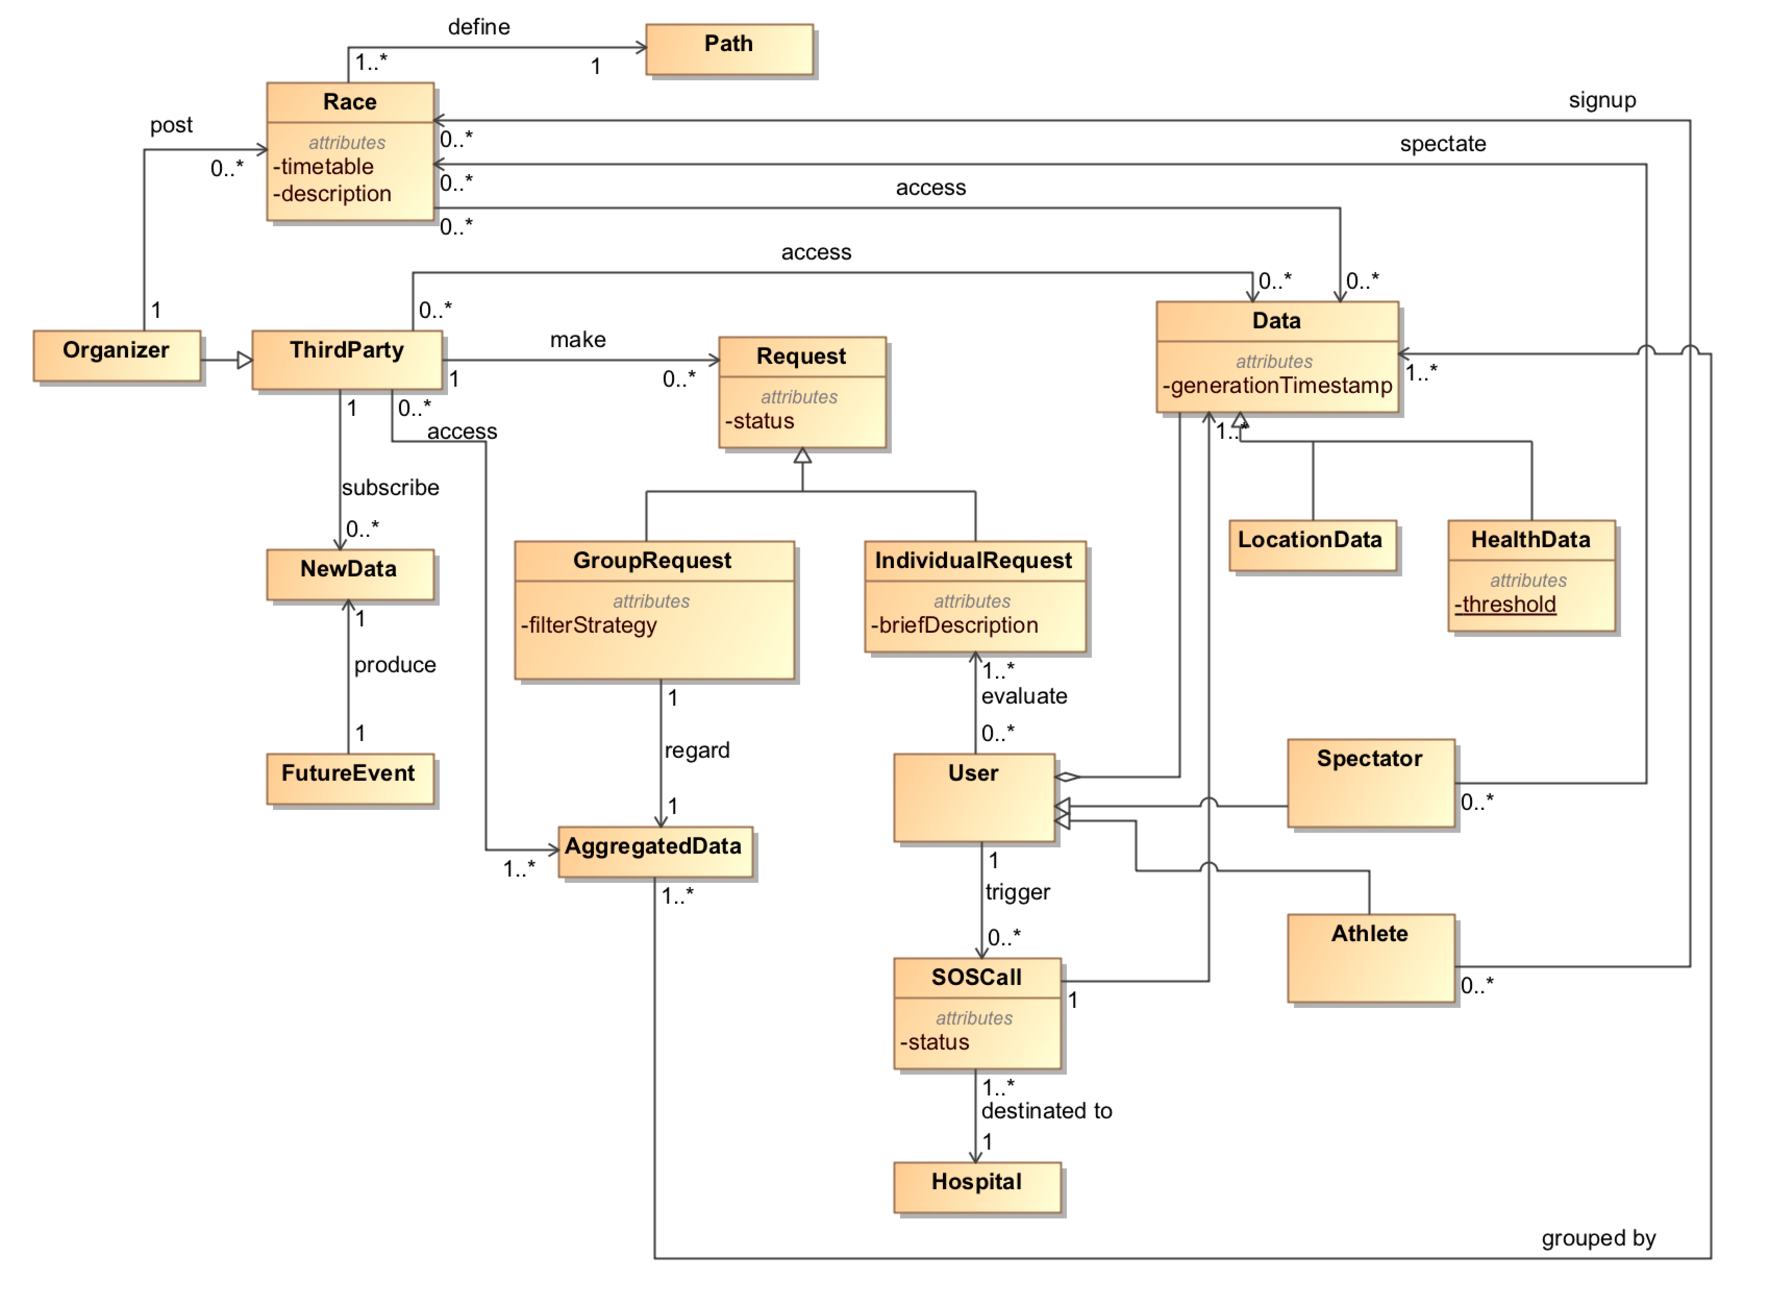
\includegraphics[width=\linewidth]{Images/classdiagram}
\caption{Class diagram of the environment}
\label{fig:classdiagram}
\end{figure}

This diagram specifies the interaction with the actors and the objects of the world. The core point of 
the environment is the data, but what should be analyzed are its entry point and exit point (i.e. usage):

\begin{enumerate}
\item Request: an entry point essential to share the data;
\item SOSCall: an very important usage for unhealthy people;
\item Race: a feature necessary for runners.
\end{enumerate}

\subsubsection{Request perspective}
Since people's data are very confidential information, a request has to be asked if someone desires it. 
Therefore, the design of how requests should work is essential. To give a better understanding of this, 
the following state diagram (Figure: \ref{fig:requestdiagram})  describes the possible states of a request:

\begin{figure}[H]
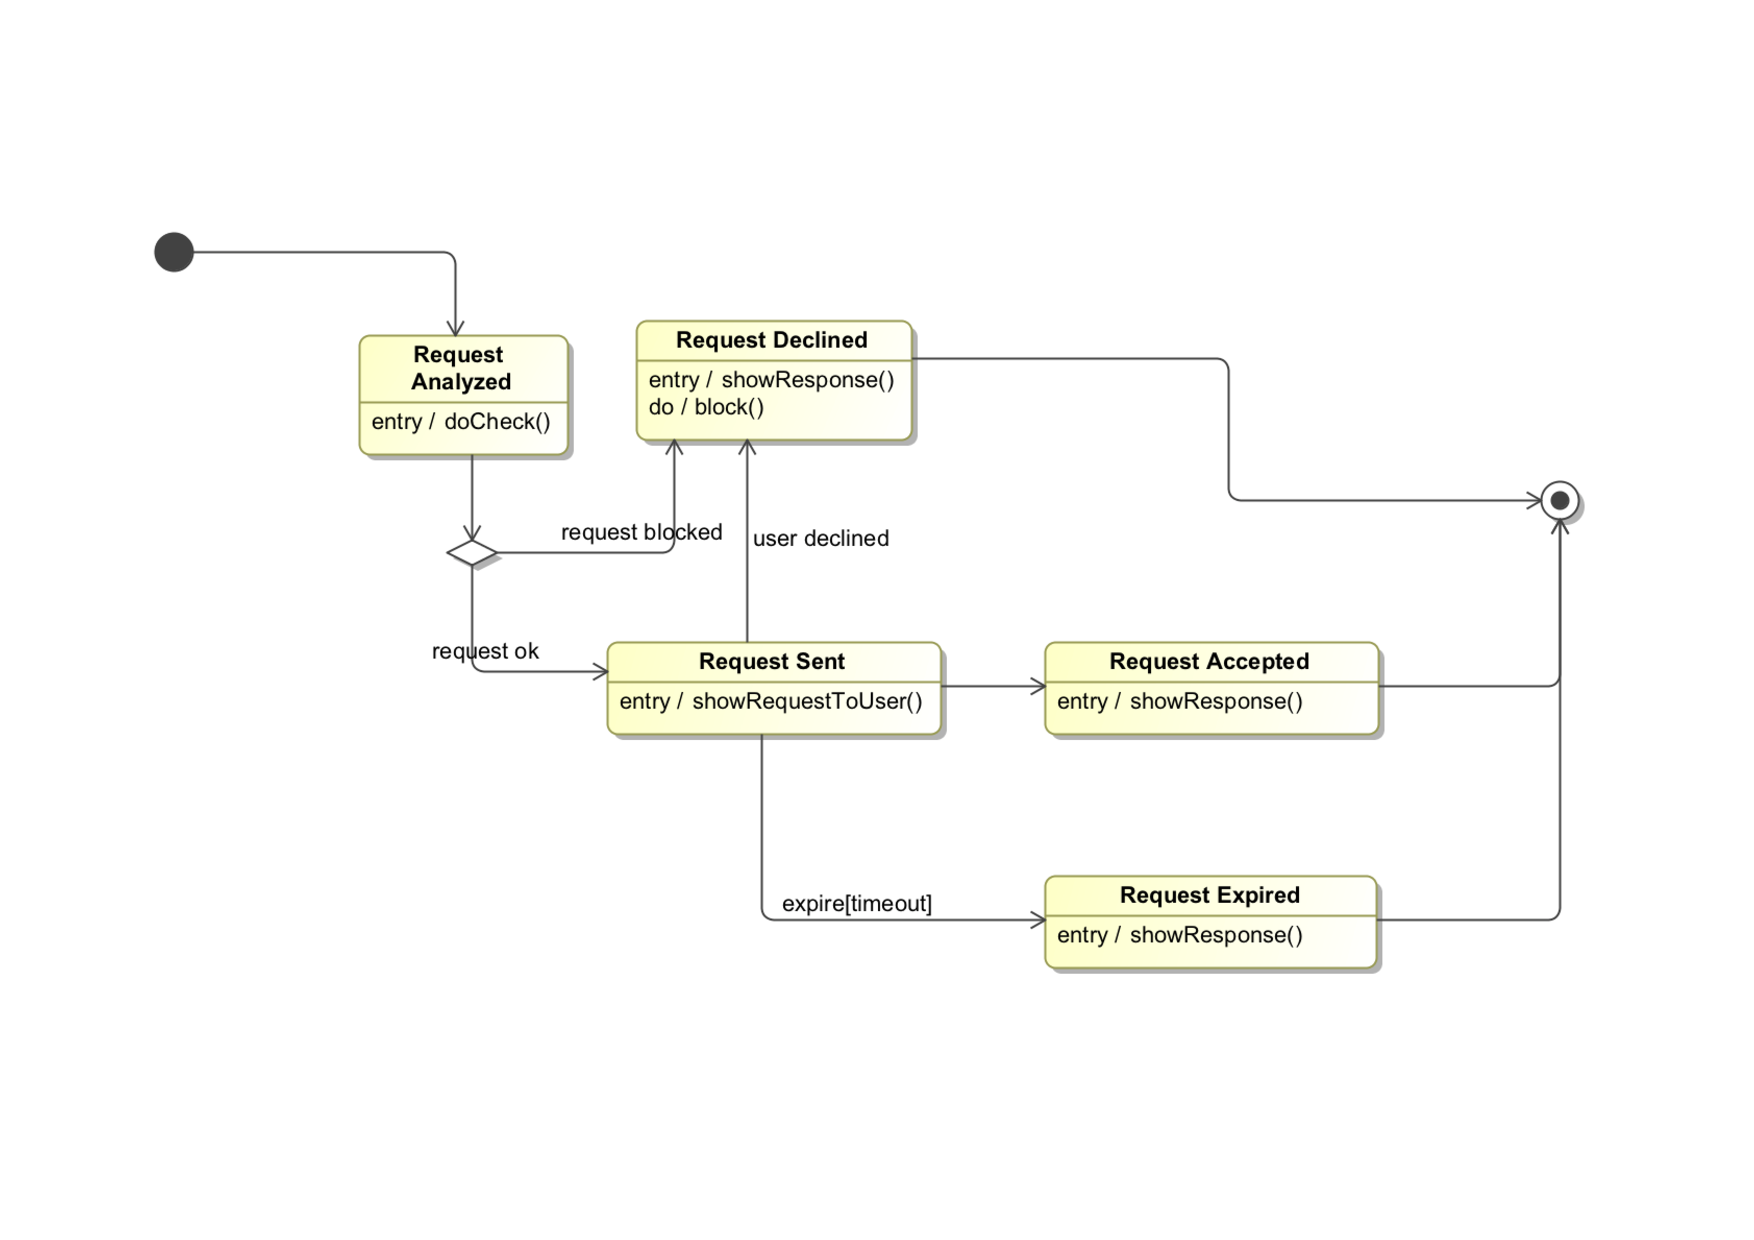
\includegraphics[width=0.8\linewidth]{Images/requestdiagram}
\caption{State diagram of a request}
\label{fig:requestdiagram}
\end{figure}

\subsubsection{SOSCall perspective}
For unhealthy people, a latency in a help call is a problem of life and death. Therefore, a better 
description of these calls is crucial. The following state diagram (Figure: \ref{fig:sosdiagram}) 
describes the possible states of a SOSCall:

\begin{figure}[H]
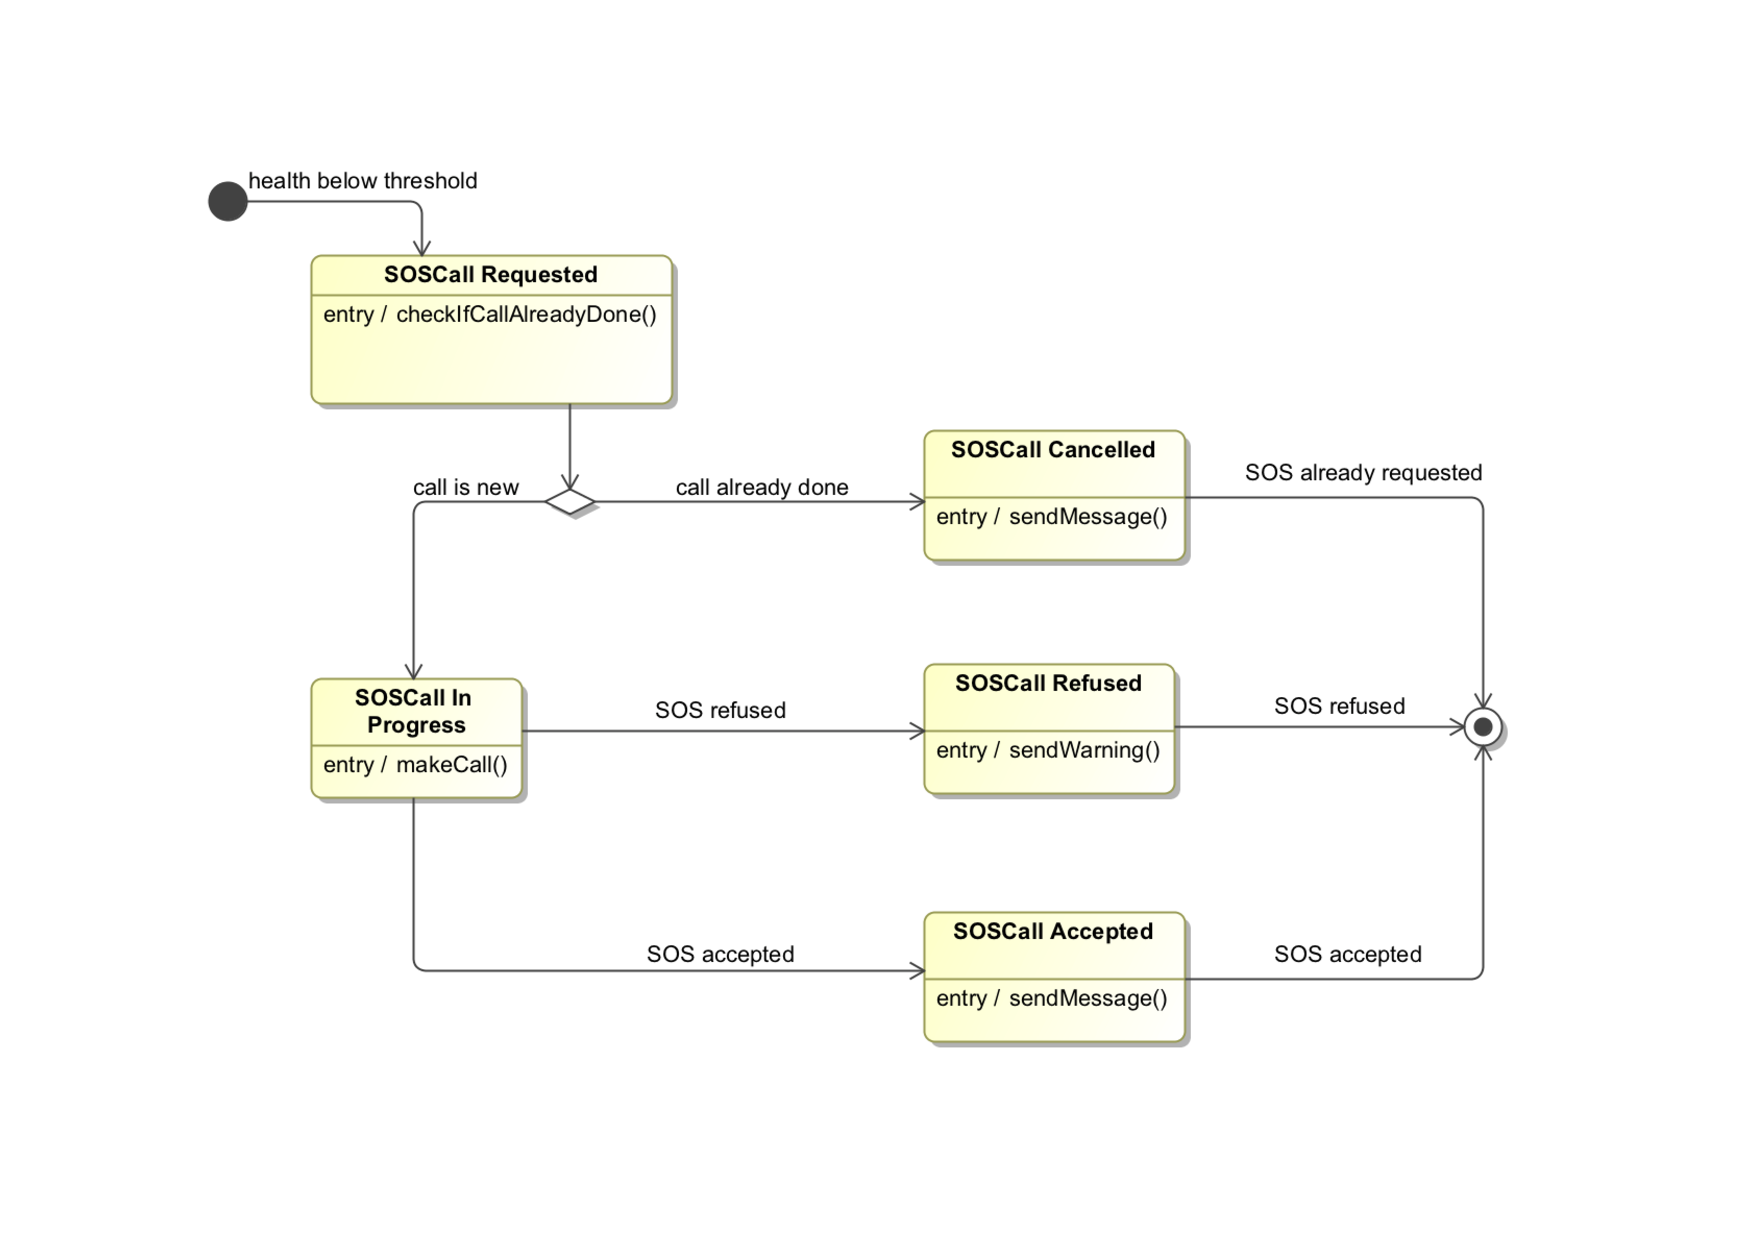
\includegraphics[width=0.8\linewidth]{Images/sosdiagram}
\caption{State diagram of a SOSCall}
\label{fig:sosdiagram}
\end{figure}

\subsubsection{Race perspective}
For someone, running is something that they cannot live without; since spectators can watch their 
position every time, it is important to describe better how a race works for better privatization of 
data. Thus, the following state diagram (Figure: \ref{fig:racediagram}) is shown: 

\begin{figure}[H]
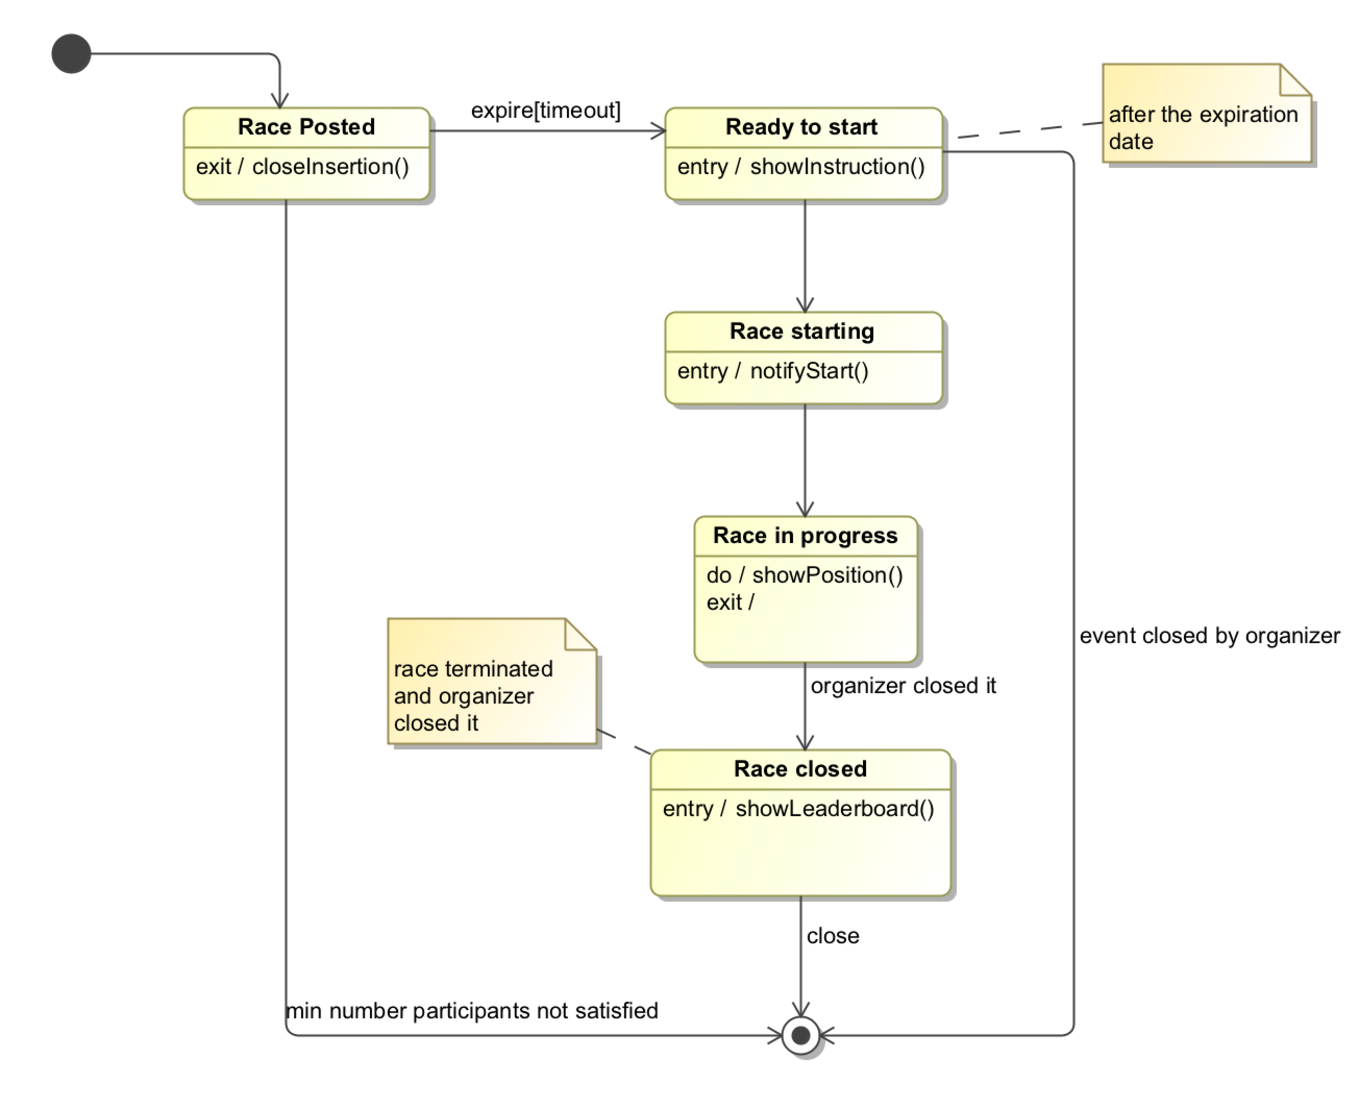
\includegraphics[width=0.8\linewidth]{Images/racediagram}
\caption{State diagram of a race}
\label{fig:racediagram}
\end{figure}